\hypersetup{pdfborder=0 0 0}

NON mais pas comp a REA2 ici.... que ce que voit signal et dans les simus d'avant, comprendre signal au truc avec lui...

Plan : dit ce qu'à fait, water mass, présente cycle de marée avec notations, présente ce que notations ISW veulent dire ie les obs M4/M5 vs M2, regarde les signaux à ce point dans VHR et situation a CS correspondantes

%-------------------------------------------------------------------------------------
\section{Campagne de mesure Gibraltar 2020 (en anglais?)}


\subsection{Déroulé campagne/chronologie}
%Section ce qui a ete fait pour preparer la campagne
In fall 2020, field campaign in the Strait of Gibraltar (and west Alboran) aboard research and survey ship L'Atalante. On site measures by the ship from 8/10/2020 to 20/10/2020 . Five moorings, two equipped with ADCP, three with CTD.. Table ... gives the period of operation and coordinate of the five moorings(Rajouter frequence).


We look at the period from 8/10 to 18/10 when both types of moorings were available/recorded, what type of signal were seen at M2, then M4 and M5.

On october ... (dates...), CTD profile of the water column were achieved as trasects at longitude ... and ... (faire carte des points)


\begin{table}[!h]
        \centering
        \begin{tabular}{|c|c|c|c|}
                \hline
                 & type & position(deg minute) & time \\ 
                 \hline
                M1 & hydro & N35 55.264 W005 46.739 & 8/10/2020 15h - 9/11/2020 12h\\
                M2 & couranto & N35 55.761 W005 45.288 & 8/10/2020 5h - 17/10/2020 15h\\
                M3 & hydro & N35 54.719 W005 44.459 & 8/10/2020 13h - 22/10/2020 21h\\
                M4 & couranto & N35 55.870 W005 41.020 & 8/10/2020 7h - 17/10/2020 14h\\
                M5 & hydro & N35 56.229 W005 41.026 & 8/10/2020 9h - 1/11/2020 14h\\
                \hline
        \end{tabular}
        %\captionof{table}{Simulation parameters}
        %\label{tab_NH-HR}
        %\end{minipage}
\end{table}


\begin{figure}[!h]
% \centering
 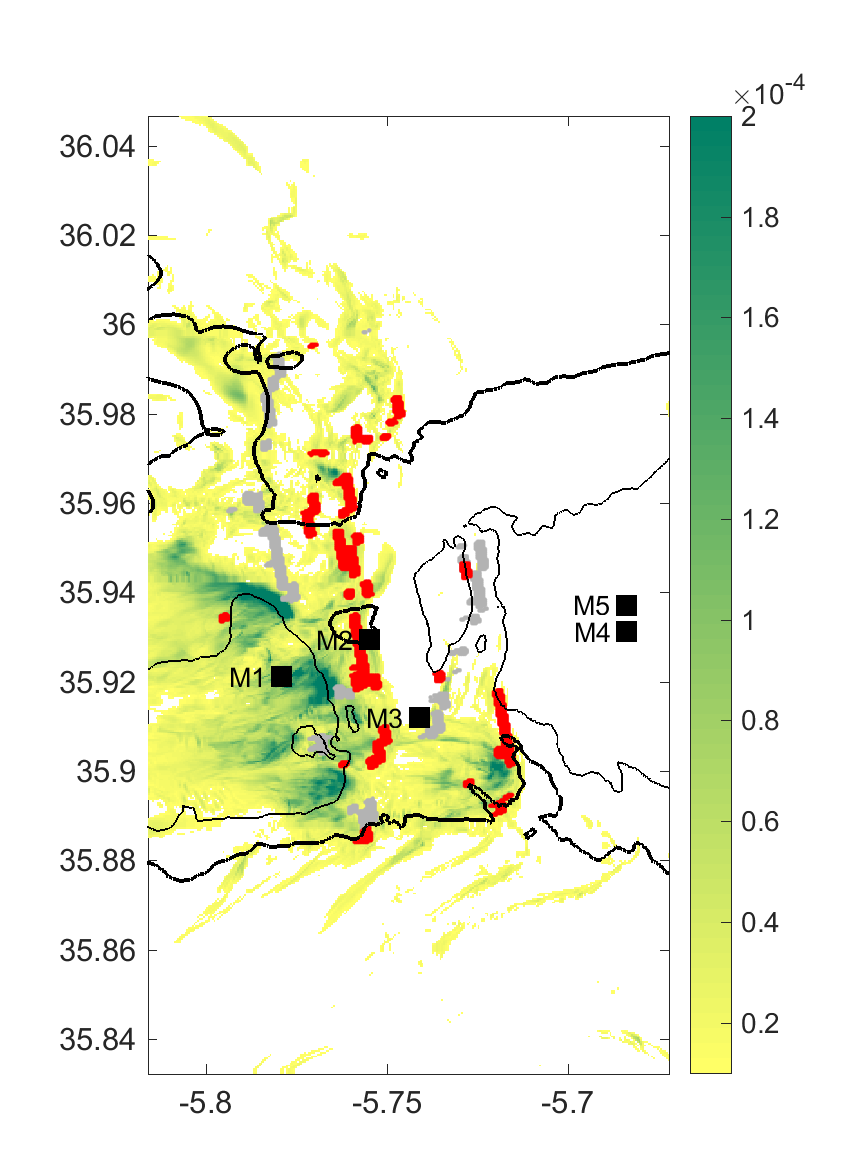
\includegraphics[width=0.4\textwidth]{./GBR3D/Fig_Moor.png}
 \caption {   }
\end{figure}


\subsection{BR*HR simulation...}



\subsection{Insights from VHR simulation, additional remarks on ISW propagation}
(carte des mouillages + traces ressauts fig avant et std Q...)

The simulatios presented in previous section were a help in preparation of the field campaogn.

Comparison with SAR data in figure shows position is alright, though form of the wave train can still differ. The speed of propagation of the ISW was used to predict position of ISW with good reslults in relation to the tidal cycle at elast in the Strait of Gibraltar. In the Alboran Sea, where the influence of the gyre is great on the form of the wave packet, prediction was not as accurate. 

Additionnally, simulated mooring data (HF outputs at coordinated) helps understand signal observed

High resolution means well resolved train of soliatry waves whereas the 2 levels imbrication not enough resolution to see this kind of well defined signal of the ISW propagation (3 way imbrication that has the moorings in its most high resolved (60m) zoom is being studied)

(Ajouter dans papier 3D : important for high resolution bathymetry at camarinal since flow over and effect of vertical compression /conservation of flux on barotropic currents that command the transition from sub to supercritical and thus the existence and form of hyd jump, especially for variety of regimen between super strong tide and neap tide weak where no jump



\subsubsection{Water mass and gyre and tide}

Juste metre les WM et dire que a la gyre, voit les images SST l'upwelling qui s'affaiblit sur période où était.  tout renversé, type d'outflow à M2)

Two series of bathysonde stations stations were realised to sample the water column, each on an end of the Strait. First on east end the 14 and 15 october, and west of the Strait the 16 of october. Figure ... presents the $\theta$-S diagram from , with each color corresponding to a different sampling station.
West, no med waters were sampled at the northenmost (ou si mais tres melange... va pas loin sur diagramme vers la bas... max salinity est 36.33) and southernmost station. East in med waters find less signal of LIW for southern station.


ontrer ubar a M2, décrire cycle neap-spring tide (les fois où courants tout renversé, type d'outflow à M2)

\subsubsection{Observations of solitons}
Arrive at neap tide part of the forthnight cycle and no solitons/nor signature of hydraulic jump are observed on moorings data until 11/10/2020 

Dire voit 4 types de signals au mouillage M4/M5 (plot force outflow (ubar M2) vs quel type signal a M4/M5) (ou 5 types : aussi bore...)

Montrer les images SAR  (un exemple et reste en annexe?)


Figure ... shows the four types of signal that are obserevd at M4 and M5, notations in figure ... indicate which type seen following the max outflow at CS. (a) is just the internal tide witha linear evolution of the interface depth and currents, noted (o). (b) still see linear evolution of currents but small amplitude interanl waves are seen that seem somewhat non-linear (L). (c) is a packet of solitary waves with somewhat well arranged waves (S). (d) is several solitary waves, that look lifke two following train each with a great amplitude leading wave (2S)

(faudrait aussi réflection? pas le temps)


Five types of signal are viewed at M4/M5, they are listed below in correspodnance with figure ... which presents the data at M4/M5 and M2, with sigils denoting correspondance to the satellite images of figure ... . Notations are indicated in parenthesis that correspond to the signal seen following the max outflow in figure ...(ubar)
\begin{itemize}
\item linear internal tide (o) : seen in figure ... where the depth of interface of density and velocity evolved linarly, during outflow upper layer still positive velocity
\item internal bore (b) : seen in figure ... , where see signal of travelling internal bore at M5 interface depth rapid evolution of 50(?)m, at M4 still see same linear evolution of velocity interface depth, at CS during outflow the upper layer velocity is near 0 or lightly negative. In the satellite SAR image in figure ... , corresponds to train of waves, the bore eventually devolves
\item small amplitude wave (L) : seen in figure ... , where there is a signal that looks life internal waves of relatively small amplitude (10m) at M5, at M4 still linear evolution of the velocity interface. At M2, as with bore case velocity upper layer null or slightly negative. Sar image in ... shows after this outflow wave travelling in Alboran, only see trace of one wave.
\item Train of solitary waves (S) : two exemples are given, in figure ... and ...  see mode 1 signal at M4, succession of troughs at M5. at M2 in both case all captors of the water column find very negative current during outflow and abrupt return to two layer. The train of figure ... corresponds to the SAR image of figure ... of train exiting the strait. Train of figure ... corresponds to RGB(?) data on which can see a hydraulic jump. using notations of previous section, it is a w-jump.
\item Train of disorganized solitary waves (2S) : Seen in figures ... and ... (where no M4 data available at time of wave's passage). As previously whole negative signal of water column at M2. See disorganized train, in fact looks like two different train following each other. In figure (2) see linked to a previous w-jump. The two trains are for the two jumps at CS... (the main one on west of sill and the eats one...)
\end{itemize}

On cases bore, ... see usually XXhours before at beginning out outflow a interfacial disturbance. 

\subsubsection{Comparison with signal in 50m simulation}
Figure ... presents the different signal at point near M4/M5 (just a bit west) in simulations SimST, SimNT and SimIT of previous section. This simulations are highly enough resolved that the train of solitary waves/bore can have devolved into a train of solitary waves by that point, and find the same types of signal except for the bore.

This time can have surafce signature at CS for all this types of signals.

Can also see maybe the signal at beginning of outflow / maybe the same.... comes from (???)

In SimNT, see o and L signal. As expected, o smooth surface. However as was pointed in previous section, in simulations at least still can have wave in Alboran. Here L is linked previously to some disturbance of surface at CS though don't trigger the ... diagnosis. see a travelling wave. Also L here see the signal in velocity of mode 1.

In simIT, S signal can be seen , linked both times to an s-jump (western jump seen over the shallowest part of the Sill)

In SimST, 2S signals although the first solitary wave that arrive(that would be linked to the eatsern jump) is low amplitude for first exemple, both are from w-jump, the difference is that the eastern jump in first case does not reach/extend as north in latitude, and could be confounded with S signal. 2nd has stronger barotropic currents at outflow


S and 2S signals are as expected linked to the jump at CS, however see an intermediate state that give L.


(SAr de SimIT c'était quoi???)




Note : classification S and 2S is very objective, S can expect that it's just both train have merged. they are linked to the form of the train. although hasn't seen on satellite an s-jump...  2S very distinct is for stronger tides, while S can be more regimes...

When look at the repartition of type of signals, see that L is more common than thought, and moreover when link to strength of barotropic current see evident link, since the hydraulic control conditions evolve.




\subsection{comp BR*HR}
(LA FLEMMMMMMMEEEEEE)
\subsubsection{Gyre and WM}

\subsubsection{tide}
aussi comparaison courant barotrope M2....

\subsubsection{Comparions of M4/M5 obs with VHR sim}
Look at simulations of the previous section and signal at mooring point teh state of the flow during the outflow at CS and the waves propagating through the area of the moorings, keep the notations of previous section.

no-jump outflow leads to the (o (or L?)), however as was presented in previous section this state may still meansolitary waves generation, they woudl have a lesser number of solitary waves as it propagates in Alboran Sea.
half jump leads to (L (or S?))  
w-jump can either elad to (S) or (2S) depending on how the first hyd jump will propagate






Comparaison avec 50m des signals que voit et lien avec ressauts

Peut pas faire comparaison du signal avec BR*HR, soliton pas assez résolu pour comprendre signal


